
\subsection{Major Documentation Deliverables}

\subsubsection{Project Charter}
The Project Charter will be maintained in a shared GitHub repository and updated after any major changes in project scope or deadlines. The initial version will be delievered on September 30th, 2024.

\subsubsection{System Requirements Specification}
The SRS will be mainainted in a shared GitHub repository and updated as required as needed in any changes in system capabilities. The document will be delivered on October 21st, 2024.

\subsubsection{Architectural Design Specification}
Architectural Design Specification will be maintained in a shared GitHub repository and updated following any changes to the system's structure. The document will be delivered on Novemeber 4th, 2024. 


\subsubsection{Detailed Design Specification}
The Detailed Design Specificationw will be maintained in a shared GitHub repository and updated if any signinficant design changes occur. The DDS document will be delivered at the end of Sprint 5 (February, 2025).

\subsection{Recurring Sprint Items}

\subsubsection{Product Backlog}
Items will be added to the product backlog based system requirements outlined in the SRS. The items will be prioritized during sprint planning meetings based on complexity and impact on ability to move forward with the project. Jira will be used to maintain and share the product baklog with team members and stakeholders.

\subsubsection{Sprint Planning}
Each sprint will be planned during a sprint planning meeting held at the beginning of the sprint cycle. There will be 8 sprints over the course of both semesters.
\subsubsection{Sprint Goal} 
The sprint goal will be decided collaboratively during the sprint planning meeting by the development team.
\subsubsection{Sprint Backlog}
The sprint backlog will be selected from the product backlog during sprint planning, focusing on the highest-priority items. The team will use Jira to maintain and track the sprint backlog and updated as needed.

%%% Jasper wrote this
\subsubsection{Task Breakdown}
Individual tasks will be partitioned into hardware, software, or group tasks, and an applicable team member will voluntarily claim uncompleted tasks. Time spent on tasks will be documented in a spreadsheet.

%%% Jasper wrote this
\subsubsection{Sprint Burn Down Charts}
The presentations will go in a rotation of four weeks, in the order of Luis, Jasper, Chris, Joshua. The person responsible for the presentation will also be responsible for the sprint burn-down chart. Individual members will be responsible for reporting their time, either directly to the spreadsheet or to the group. The following figure is an example of the burn down chart.

\begin{figure}[h!]
    \centering
    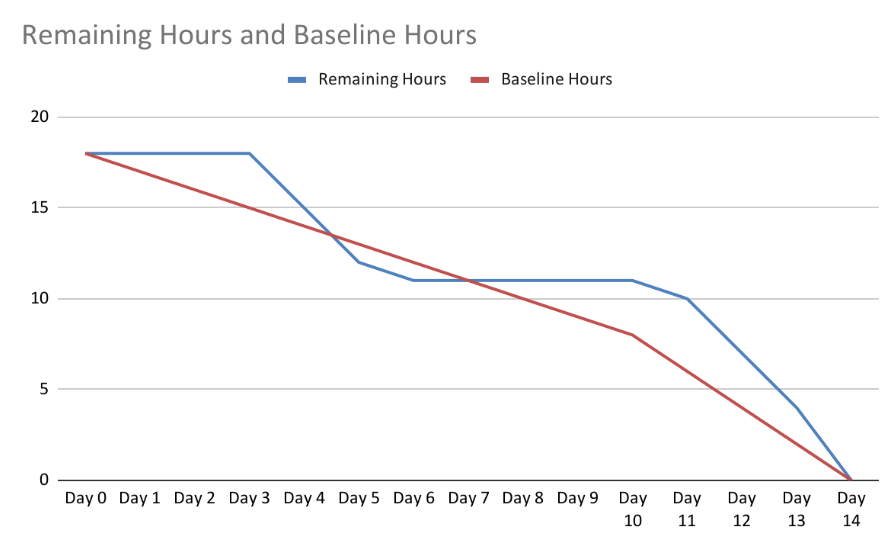
\includegraphics[width=0.5\textwidth]{images/burndown}
    \caption{Example sprint burn down chart}
\end{figure}

\subsubsection{Sprint Retrospective}
How will the sprint retrospective be handled as a team? When will this discussion happen after each sprint? What will be documented as a group and as individuals, and when will it be due?

\subsubsection{Individual Status Reports}
The sprint retrospective will be conducted as a team discussion at the end of each sprint. This meeting will reflect on success and areas for improvement, with team members documeneting individual feedback. The key items will be the ways to improve, what did not work, and what did work well.

\subsubsection{Engineering Notebooks}
At a minimum the engineering notebook will be updated once during a sprint by each team member. The minimum amount for each interval is a quarter page, keeping each member accountable by documenting their input for each entry.

\subsection{Closeout Materials}

\subsubsection{System Prototype}
The final system prototype will include the complete integration fo the RV8 robot with a gripper and palletizing application. The prototype will be demonstrated by the RV8 robot palletizing boxes in ERB 335 in April 2025.
\subsubsection{Project Poster}
The project poster will include the project description, system architecture, results, and impact. It will follow standar poster dimesions (36"x48") and will be delivered in April 2025.

\subsubsection{Web Page}
The project webpage will include the project description, system requirements, demonstration videos, and deliverables. It will be provided at closeout in April 2025.

\subsubsection{Demo Video}
The video will show the RV8 robot in action performing palletizing tasks. B-reel footage will also be included for future video cuts. The video will be approximately 3-8 minutes long covering system setup, algorithms, and functionality.
\subsubsection{Source Code}
Source Code will be maintained using GitHub for version control. Source code will be provided to the customer, with licesnse terms listed in a single readme file.

\subsubsection{Source Code Documentation}
Documentation will be generated using Doxygen, provided in both PDF and browsable HTML formats.

\subsubsection{Hardware Schematics}
The hardware schematics will include wiring diagrams and any PCB layouts required for the integration of a gripper. 

\subsubsection{CAD files}
The project may involve designing and printing a gripper, in which case SolidWorks will be used for design, and final files will be provided in STL and STEP formats.
\subsubsection{Installation Scripts}
The team will deploy the software for the customer, handling any installation.

\subsubsection{User Manual}
A detailed user manual will be provided including setup steps in digital PDF format, alongside a setup video demonstrating how the robot works. 